\chapter{System Design and Implementation}
\label{ch:implementation}

\section{Software Architecture}
SwarmFlow is an independent Python~3.12 package built on the open-source libraries NumPy, Gymnasium, PettingZoo
and PyTorch. Simulation, learning, evaluation and
visualisation are separated into the modules listed in Table~\ref{tab:modules}. The environment implements the
PettingZoo parallel API: \texttt{reset} returns one observation per drone, and \texttt{step} receives one
action per drone and returns per-drone observations, rewards, termination and truncation flags. The simulator
state can be captured and restored, which is used for collision-state replay. The package is covered by 40
automated unit tests (all passing), including checks of swept collisions at high speed, immutable slot
assignment, recovery timing, reward bounds, attention permutation invariance, squashed-Gaussian
log-probabilities and time-limit handling in GAE.

\begin{table}[htbp]
\centering
\caption{Modules of the SwarmFlow implementation}
\label{tab:modules}
\small
\begin{tabularx}{\textwidth}{@{}lX@{}}
\toprule
Module & Responsibility\\
\midrule
\texttt{config.py}, \texttt{scenarios.py} & environment defaults; target paths, crossing-object generator, formation geometries, seeded scenarios\\
\texttt{env.py} & \texttt{SwarmEnv}: flight model, local observations, swept collisions, reward, recovery and episode metrics\\
\texttt{policy.py} & set encoders, shared actor--critic network, checkpoint loading for inference\\
expert planner & sampling-based model-predictive planner used to generate demonstrations\\
\texttt{train.py} & DART/DAgger imitation, parallel rollouts, reward scaling, GAE, PPO update, validation\\
\texttt{curriculum.py} & three-stage resumable training pipeline and held-out test of the selected model\\
\texttt{evaluate.py}, \texttt{suite.py} & episode runner, aggregate metrics, selection score and acceptance criteria\\
\texttt{server.py}, \texttt{web/} & local HTTP server and browser flight laboratory (HTML, JavaScript canvas)\\
\texttt{cli.py} & command-line entry points \texttt{view}, \texttt{eval}, \texttt{train}, \texttt{pipeline}\\
\bottomrule
\end{tabularx}
\end{table}

\section{Training Pipeline}
Figure~\ref{fig:curriculum} shows the complete training pipeline. Stage~1 learns formation keeping with a
static, moving and turning target; stage~2 adds lateral and head-on objects; stage~3 adds repeated crossings
and the wind gust. Inside every stage, four demonstration rounds (one DART round and three DAgger rounds) are
followed by validation of the initialised policy, ten critic warm-up updates and PPO fine-tuning. Rollouts are
collected from eight environment instances whose neural-network inference is batched: each update uses
$8 \times 256 \times 8 = 16{,}384$ drone transitions. Every update writes a resumable checkpoint, so an
interrupted run continues where it stopped.

\begin{figure}[htbp]
  \centering
  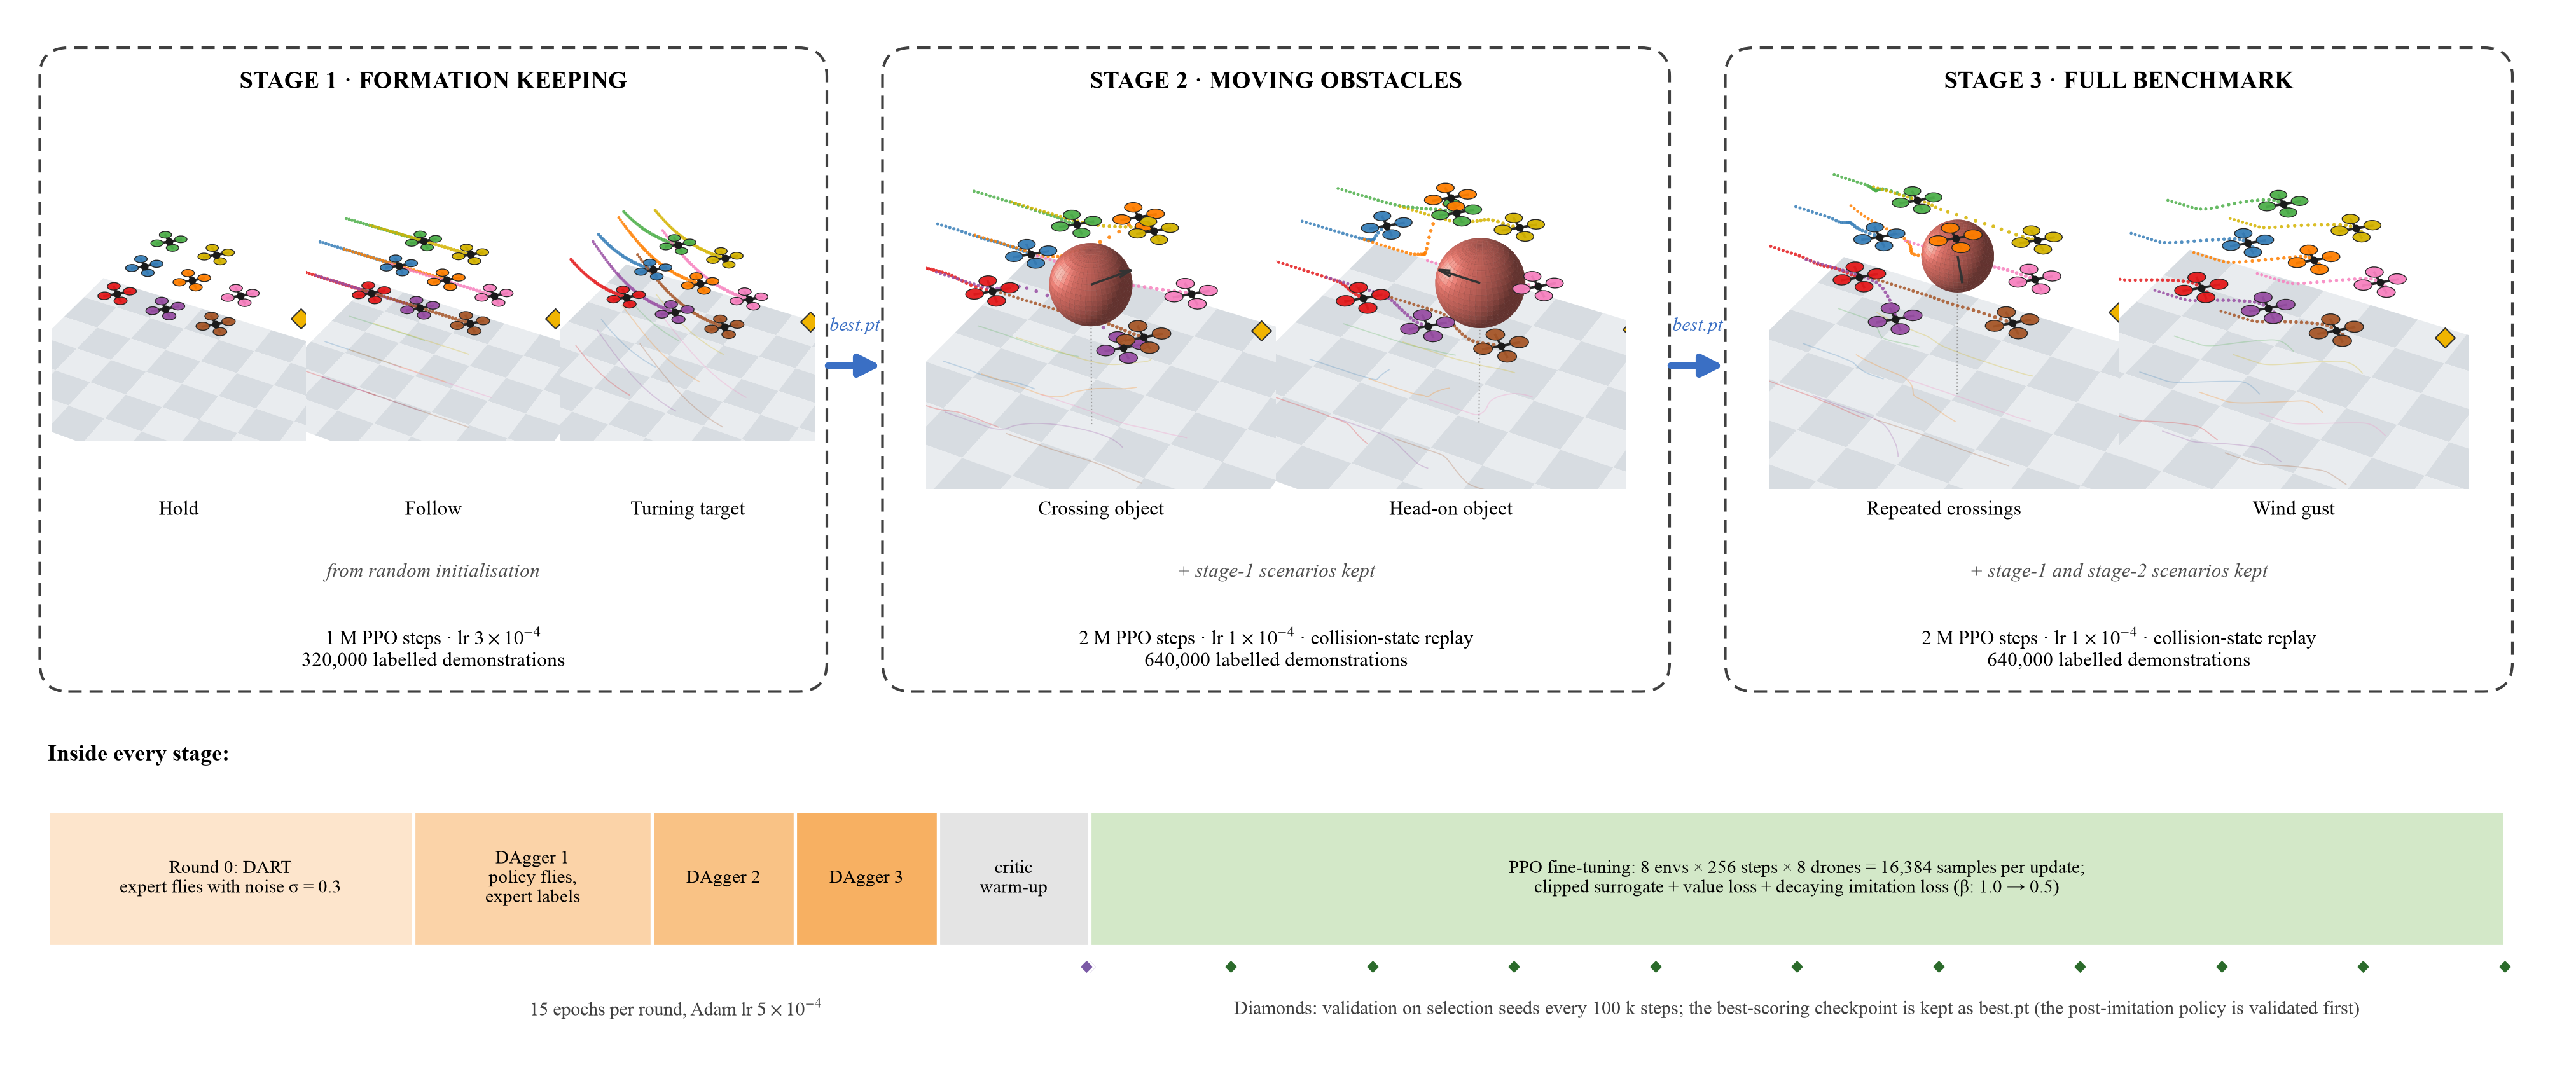
\includegraphics[width=0.88\textwidth]{fig_curriculum}
  \caption[Three-stage curriculum training pipeline]{Three-stage curriculum. Each stage adds harder scenarios
  (thumbnails rendered from the simulator), keeps the earlier ones and starts from the best checkpoint of the
  previous stage. The bar shows the phases inside every stage.}
  \label{fig:curriculum}
\end{figure}

\section{Training Configuration}
Table~\ref{tab:hyper} lists the configuration of the final model. The complete PPO budget is
$5\times10^{6}$ environment steps, i.e.\ $4\times10^{7}$ individual drone decisions. The PPO phases of the
three stages took 1{,}925\,s, 3{,}904\,s and 3{,}999\,s (about 2.7\,h in total) on a laptop at roughly
550--570 environment steps per second.

\begin{table}[htbp]
\centering
\caption{Training configuration of the final model}
\label{tab:hyper}
\footnotesize
\setlength{\tabcolsep}{4pt}
\begin{tabular}{@{}llll@{}}
\toprule
Setting & Value & Setting & Value\\
\midrule
PPO steps (stage 1/2/3) & 1\,M / 2\,M / 2\,M & Learning rate (stage 1 / 2--3) & $3\!\times\!10^{-4}$ / $1\!\times\!10^{-4}$\\
Parallel environments & 8 & Rollout horizon & 256 steps\\
Samples per update & 16{,}384 & Epochs / minibatch & 5 / 2{,}048\\
Discount $\gamma$ / GAE $\lambda$ & 0.99 / 0.95 & Clip $\epsilon$ / KL limit & 0.2 / 0.03\\
Initial / minimum action std & 0.20 / 0.05 & Entropy coefficient & 0\\
Imitation weight $\beta$ & 1.0 $\to$ 0.5 & Gradient clip (actor, critic) & 0.5, 0.5\\
Demonstration rounds & 4 (15 epochs each) & Demonstration steps per round & 10\,k (stage 1), 20\,k\\
Labelled samples (stage 1/2/3) & 320\,k / 640\,k / 640\,k & Expert margins (soft / hard) & 0.6\,m / 0.25\,m\\
Validation & every 100\,k steps & Selection seeds & 10 per scenario\\
Optimiser & Adam, $\varepsilon = 10^{-5}$ & Network width & 128\\
\bottomrule
\end{tabular}
\end{table}

\section{Web-Based Flight Laboratory}
To demonstrate and inspect the learned behaviour, the project includes a browser-based flight laboratory
(Figure~\ref{fig:viewer}). A local Python server runs the simulation and exposes a small REST interface
(\texttt{/api/state}, \texttt{/api/reset}, \texttt{/api/step}, \texttt{/api/inject}); the page renders the
actual three-dimensional simulation state on an HTML canvas. The user can select the scenario, formation
geometry, number of drones and seed, start and pause a flight, orbit the camera or switch to side and top
projections, and inject additional crossing or head-on objects with chosen speed and radius at any time. Live
panels show the slot error, the minimum surface clearance, the number of recovered disturbances and the flight
state. A second panel reports the training history and the held-out test of the loaded model. The viewer only
executes the saved network weights; it does not modify them.

\begin{figure}[htbp]
  \centering
  
\includegraphics[width=0.6\textwidth]{viewer/viewer_overview}
  \caption[SwarmFlow web flight laboratory running the final model]{SwarmFlow web flight laboratory running the
  final model (crossing scenario, held-out seed 100000, $t = 8.3$\,s). Left: mission and disturbance controls;
  centre: 3-D view with drones (numbered), assigned slots (squares), reference target and object; bottom: live
  metrics and slot-error timeline.}
  \label{fig:viewer}
\end{figure}
